\section{"不变量"的求解方法}
下面给出引题的证明.
\begin{proof}[引题的证明]\footnote{此证明出自AOPS,由罗老师整理及翻译.}\footnote{这证明不包括构造过程,请参考本文附录.}
记奇数号碗中苹果和梨的总数分别为$A_1,P_1$,偶数号碗的苹果和梨的总数分别为$A_2,P_2$.
由于$(i-j)$时偶数,故每次操作都是将奇(偶)数号碗中的一个梨和苹果换到偶(奇)数号碗中,于是$(A_1-A_2)$
与$(P_1-P_2)$同时增加$2$或$-2$,这表明\begin{equation}
    M=(A_1-A_2)-(P_1-P_2)\label{eqn:inv}
\end{equation}
是本题合法操作的不变量.若$ab$为奇数,则$a,b$皆为奇数,初始状态下由\eqref{eqn:inv}
得$M=1-(-1)=2$,结束时$M=-1-1=-2$,由$M$为不变量推出矛盾,命题获证.
\end{proof}

此题的证明充分的利用了不变量的性质(就是说,它是不会变的),从而推出矛盾.事实上,在代数问题中
不变量亦是极其有用的.
\begin{problem}\footnote{出自:奥数教程(八年级),\S{8},例5.有改动.}
    已知三个数89,12,3,进行一种运算$Q$:\label{pbl:qar}
    \begin{equation}
        Q(a,b,c)=(\dfrac{a+b}{\sqrt{2}},\dfrac{a-b}{\sqrt{2}},c^2.)\label{eqn:qar}
    \end{equation}
    问:能否经过若干次运算$Q$,得到3个数90,14,10?证明它.
\end{problem}
此题初看没有头绪,而此类问题的一般解法是从\eqref{eqn:qar}中寻找不变量.
\begin{proof}
    \kaishu{答案显然是否定的.接下来给出证明.}
    \songti 我们知道
    \begin{equation}
        \left(\dfrac{a+b}{\sqrt{2}}\right)^2+\left(\dfrac{a-b}{\sqrt{2}}\right)^2+c^2=a^2+b^2+c^2.\label{eqn:eqv}
    \end{equation}
    \eqref{eqn:eqv}就是说,经过一次运算$Q$之前与之后的三个数的平方和是不变的.至此,我们找到了此题中的"不变量":平方和.
    而$${89}^2+12^2+3^2=8074,$$
    $$90^2+14^2+10^2=8396>8074.$$
    故经过题中题中规定的运算不能由已知的三个数得到$90,14,10$三个数.
\end{proof}
从上两例中我们可以看出"不变量"实际上是一种思想,要找到并证明它需要的是各种数学方法,如判别式,恒等变形等.下面分几类详细讨论.
\subsection{一般不变量}
\begin{problem}\footnote{选自罗老师提供的资料.}
    在某部落的语言中一共只有两个字母$A$与$B$,并且该语言具有以下性质:
    如果从单词中删去相邻的字母串$AB$,词义保持不变.或者说:单词中添加字母串$BA$
    或$AABB$,词义保持不变.

    问:$ABB=BAA$吗?
\end{problem}
\begin{solution}
    记每个单词为$(a,b)$,其中,$a$为该单词中$A$的个数,$b$为该单词中$B$的个数.
    现寻找"不变量".显然,在一串"保义变换"中的$a-b$都是不会变的.而$$ABB:(1,2),1-2=-1;\quad BAA:(2,1),2-1=1.$$
    故$$ABB\neq BAA.$$
\end{solution}
在此题中由于原本的条件是不足以使用的,因为字母数太少了,故考虑寻找"不变量".

在寻找不变量的过程中,我们需要在变量之中看出规律来.如题\ref{pbl:qar},是从无理式(准确的来说,是根式)中寻找规律;
在此类题目中,我们需要求运算前的三个数与运算后的三个数的$n$\footnote{此$n$是根式的次数.例如,在题\ref{pbl:qar}中,就是通过求其平方和.}次方和的关系.
\subsection{多项式中的"不变量"}
\subsubsection{判别式}
在下一题中,我们会发现纯粹的寻找不变量的方法是无用的;我们必须通过寻找判别式中的规律
中的不变量来寻找答案.
\begin{problem}
    对于二次三项式$ax^2+bx+c$,允许做下面的运算:
    \begin{enumerate}
        \item 将$a$与$c$对换;
        \item 把$x$换成$(x+t)$,其中,$t$为任意实数.重复作这样的运算,能把$x^2-x-2$换成$x^2-x-1$吗?
    \end{enumerate}
    重复作这样的运算,能把$x^2-x-2$换成$x^2-x-1$吗?
\end{problem}
\begin{solution}
    我们考虑判别式$\Delta$.第一种运算显然不改变$\Delta$.第二种运算不改变多项式两根之差.现有$$\Delta=b^2-4ac=a^2\left[\left(\dfrac{b}{a}\right)^2-4\dfrac{c}{a}\right]$$,而$-\dfrac{b}{a}=x
    _1+x_2$,$\dfrac{c}{a}=x_1x_2$,从而$\delta=a^2\left( x_1-x_2 \right)^2.$即第二种运算不改变$\delta.$而两个二次三项式的判别式为$9$与$5$,不能达到.
\end{solution}
\subsubsection{整式的加减}
\begin{problem}\footnote{选自罗老师提供的资料.}
    若多项式$f(x),g(x)$分别为:
    \begin{enumerate}
        \item $f(x)=x^2+x,g(x)=x^2+2;$
        \item $f(x)=2x^2+x,g(x)=2x;$
        \item $f(x)=x^2+x,g(x)=x^2-2;$
    \end{enumerate}
    用\textbf{加,减,乘}能否从$f(x),g(x)$中得$h(x)=x?$
\end{problem}
\begin{solution}
    对$f,g$用这三种运算,我们得到多项式\begin{equation}\label{eqn:pol}
        P(f(x),g(x))=x,
    \end{equation}
    它应该对任意$x$成立,对于(1),(2),我们给出特定的$x$的值,使\eqref{eqn:pol}不成立.
    \begin{enumerate}
        \item 在(1)中$f(2)=g(2)=6,$在对6反复用三种运算时,总是得到6的倍数,但\eqref{eqn:pol}的右边是2.
        \item 在(2)中$f(\dfrac{1}{2})=g(\dfrac12)=1$,\eqref{eqn:pol}左边为整数,右边为分数.
        \item 在(3)中$$(f-g)^2+2g-3f=x.$$
    \end{enumerate}
    
    
\end{solution}
\subsection{奇偶不变量与余数不变量}
在一些情况下,我们不能找到恒为定值的量,但我们可以考虑模算术.常见的模有:$2$(奇偶性),$4$(平方数的判断)等.
接下来分一些模型来讨论.
\subsubsection{存取模型}
所谓"存取模型"是指在某些物品在被使用去某些数量后会自动填充,求最后会不会用完.这种题目主要是通过同余的方法来解决.

下一道题中就是通过$\pmod 3$找出不变量,并解决问题.
\begin{problem}
    一条龙有100个头.一名武士一剑可以砍掉它的15,17,20或5个头,就在这四种情况下,在龙的肩上又分别会长出24,2,14或17个新的头.如果把头都砍光时,龙就死了.龙会死吗?
\end{problem}
\begin{solution}
    \kaishu{显然是不会的,下面给出证明.}\songti
    由于$$15-24\equiv 17-2\equiv 20-14\equiv 5-17\equiv 0\pmod3,$$故头$\mod 3$的余数不会变.而$100\equiv 1\pmod3,$龙不会死.
\end{solution}
\subsubsection{博弈模型}
在不变量原理中的博弈模型就是指从任意一种初状态皆能到最终状态的可能性.

下一道题中就是通过$\pmod 2$找出不变量,并解决问题.
\begin{problem}
    一个圆分为6个扇形(图\ref{fig:side:b}).每个扇形中放有一枚棋子.每一步允许将任何两枚棋子分别移入相邻的扇形.试问,能否通过这种操作,把6枚棋子全都移到一个扇形之中?
    \begin{figure}
        \begin{minipage}[t]{0.5\linewidth}
        \centering
        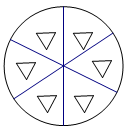
\includegraphics{graphics/circ1.png}
        \caption{初始状态}
        \label{fig:side:a}
        \end{minipage}%
        \begin{minipage}[t]{0.5\linewidth}
        \centering
        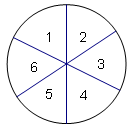
\includegraphics{graphics/circ2.png}
        \caption{分析}
        \label{fig:side:b}
        \end{minipage}
        \begin{minipage}[t]{0.5\linewidth}
            \centering
            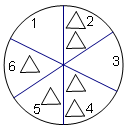
\includegraphics{graphics/circ3.png}
            \caption{移动后状态}
            \label{fig:side:c}
            \end{minipage}
        \end{figure}
        
\end{problem}
\begin{solution}
    不能.设第$n$个扇形中有棋子$p_n$个.考察量$$
        M:=\sum n\cdot p_n
    $$
    在将一枚棋子移入相邻的扇形中时$M$的奇偶性改变了.这说明每一次移动时$M\pmod2$不变.
    但是,$$M_\text{初始}=21,\quad M_\text{目标}=6N(N\in\mathbb{Z}^{+}).$$21不被6整除,故目标不能达成.
\end{solution}
\subsection{半不变量:函数的单调性与有界性}
在某些"连续"的问题中,例如函数问题中,我们的初始值与目标可能超出整数范围\footnote{需要指出的是,在整数域内一般不变量与取余也有可能解决不了问题.},甚至于扩大到全部实数域.这时,余数与一般不变量都起不了作用;我们可以通过寻找问题中单调变化的量以及有界的量\footnote{从高等数学的角度,函数的单调性与有界性是紧紧的联系着的:例如,$f(x)$在$\mathcal{X}$内单调递增,其导函数$$f^{\prime}(x)=\dfrac{dy
}{dx}(x)$$恒大于0.}从而解决问题.